
\Problem{Trees --- Recursive traversal}

\Statement

Write a program that reads the description of a natural binary tree
and prints its postorder and inorder traversals.

\medskip

The description of a tree
consists of its traversal in
preorder, which includes the leaves marked with a -1.

\medskip

For instance, the tree

\begin{center}
\begin{latexonly}
  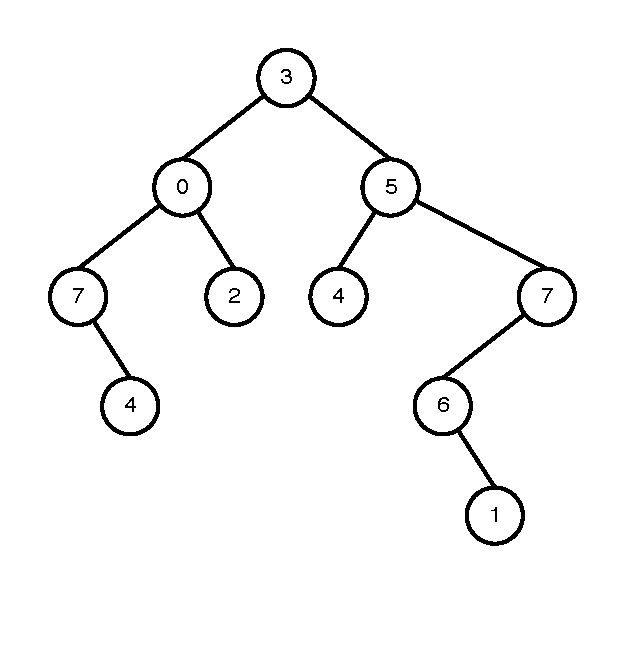
\includegraphics[height=6cm]{tree.pdf}
\end{latexonly}
\begin{htmlonly}
  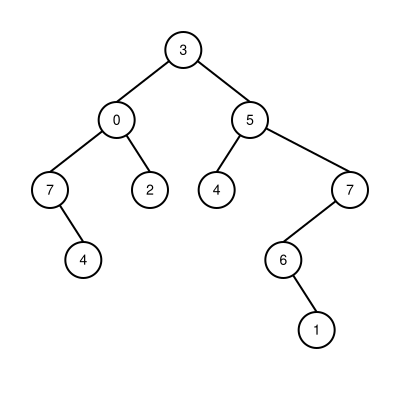
\includegraphics[height=6cm]{tree.svg}
\end{htmlonly}
\end{center}

would be described as
{\tt \small
\quad 3 0 7 -1 4 -1 -1 2 -1 -1 5 4 -1 -1 7 6 -1 1 -1 -1 -1
\normalsize
}

\Input

Input consists of the description of a natural binary tree.



\Output

Your program must print two lines, with the postorder and inorder traversals of the tree.
Follow the format in the samples.



\SampleOneCol
